%%
%  ******************************************************************************
%  * #file    Szablon_raportu_EN_Latex.tex
%  * #author  Adrian Wójcik   adrian.wojcik(at)put.poznan.pl
%  *          
%  * #commit  Patryk Kościk   koscikpatryk(at)gmail.com
%  *          Modified the template for Projekt przejsciowy purposes          
%  *          
%  * #version 1.0
%  * #date    09-Mar-2022
%  * #brief   PROJPRZEJ
%  *
%  ******************************************************************************
%%  
\documentclass[11pt, a4paper]{article}

\usepackage{SM_template}

% Wypełnijcie te dyrektywy zgodnie z waszym tematem
% \lab      -> NAZWA CZUJNIKA, np.: 'DHT22'
% \comment  -> Króciutki opis co to, np.: 'Cyfrowy budżetowy czujnik temperatury'
%
\lab{Moduł KY-021}
\comment{Kontaktron, normalnie otwarty łącznik elektryczny sterowany polem magnetycznym}

% Absolutny zakaz dotykania tego tutaj bo jak dotkiecie to coś jebnie
\university{Politechnika Poznańska}
\faculty{Wydział Automatyki, Robotyki i Elektrotechniki}
\institute{Instytut Robotyki i Inteligencji Maszynowej}
\department{Zakład Sterowania i Elektroniki Przemysłowej}
\addbibresource{bib/Kontaktron-KY-021.bib}
\nocite{*}


%%
%
% Początek dokumentu
%
%%
\begin{document}

%% Strona tytułowa %%
\mainpage{{Kontaktron-KY-021/zdj_modułu/foto_2.jpg}}
\newpage

\section{Opis elementu} \addcontentsline{toc}{section}{Wstęp}
Głównym elementem modułu jest kontaktron, czyli łącznik elektryczny, wykorzystujący podatność przewodów, znajdujących się w szklanej ampułce, na pole magnetyczne. Funkcjonalnie odpowiada on działaniu przycisku monostabilnego (kontaktron pozostaje zamknięty tak długo jak znajduje się w polu magentycznym).% Opisywany moduł zbudowany jest z trzech pinów, kontaktronu i rezystora $10k\Omega$. Całość jest odpowiednio zamontowana do płytce drukowanej.

\vspace{0.3cm}
\begin{figure}[h]
\centering
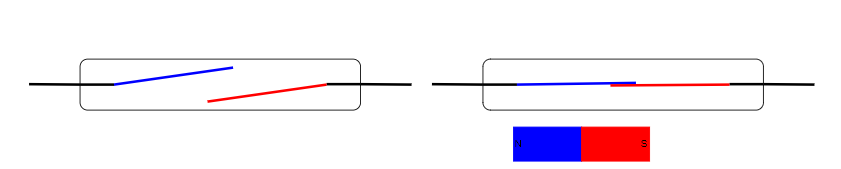
\includegraphics[width=.8\linewidth]{fig/Kontaktron-KY-021/zasada_dzialania/zasada_dzial.png}
\caption{Działanie kontaktronu: po lewej styki rozwarte (brak działania pola magnetycznego), po prawej styki zwarte (pod wpływem zewnętrznego pola magnetycznego (magnesu)) \cite{reed_jpeg_schematic}}
\label{fig:sub1}
\end{figure}
\vspace{0.3cm}

\subsection{Zasada działania}
Zasada działania kontaktronu, będącego głównym elementem modułu KY-021, polega na zbliżeniu do siebie dwóch styków znajdujących się wewnątrz szklanej ampułki przy pomocy zewnętrznego pola magnetycznego (najczęściej jest to po prostu magnes), w konsekwencji zamykając obwód. Opisywany moduł zbudowany jest z trzech pinów, kontaktronu i rezystora $10k\Omega$. Całość jest umieszczona do płytce drukowanej.

\vspace{0.2cm}
\begin{figure}[h]
\centering
\begin{subfigure}{.5\textwidth}
  \centering
  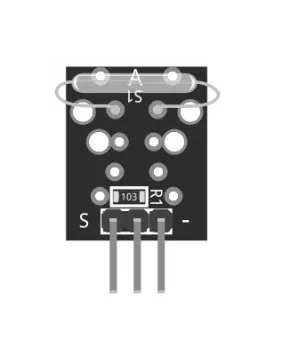
\includegraphics[width=.65\linewidth]{fig/Kontaktron-KY-021/zdj_modułu/ky-021.jpg}
  \caption{Ilustracja modułu \cite{KY_021_example_photo}}
  \label{fig:sub1}
\end{subfigure}%
\begin{subfigure}{.5\textwidth}
  \centering
  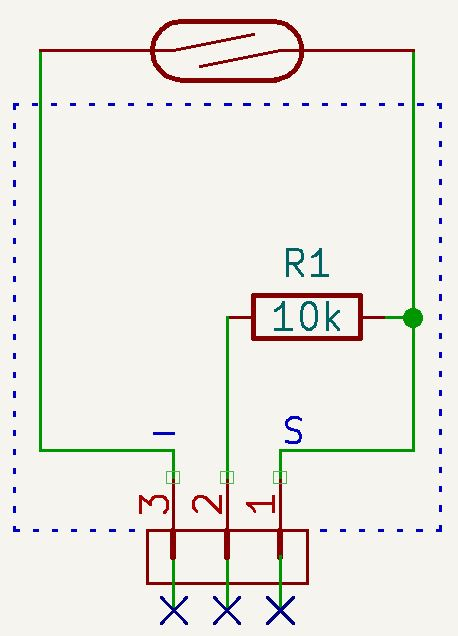
\includegraphics[width=.65\linewidth]{fig/Kontaktron-KY-021/polaczenie_modulu/schemat_ky_021.png}
  \caption{Schemat modułu}
  \label{fig:sub2}
\end{subfigure}
\label{fig:test}
\end{figure}
\vspace{0.2cm}

\subsection{Zastosowania}
Najczęstszym zastosowaniem kontaktronu są systemy alarmowe, w których kontaktron umieszcza się na oknach/drzwiach. W momencie ich otwarcia zostaje przerwany obwód, co jest rejestrowane przez odpowiedni system. Innym zastosowaniem jest szeroko pojęta robotyka i automatyka przemysłowa, gdzie kontaktronów używa się do pozycjonowania ramienia robotycznego lub taśmociągu.


\newpage

\section{Implementacja czujnika}
Ogólny schemat elektryczny modułu KY-021 przedstawiono poniżej. Dzięki takiemu układowi połączeń czujnik kontaktronowy można podłączyć do mikrokontrolera na dwa sposoby: w konfiguracji z rezystorem podciągającym (pull-up) lub w konfiguracji z rezystorem ściągającym (pull-down). Należy także zwrócić uwagę na to, że poszczególne modele czujnika mogą mieć zamienione kolejności pinów (zamieniony pin S (1) z pinem ''-'' (3))

\subsection{Połączenie fizyczne}

\vspace{0.5cm}
\begin{figure}[H]
\centering
\begin{subfigure}{.5\textwidth}
  \centering
  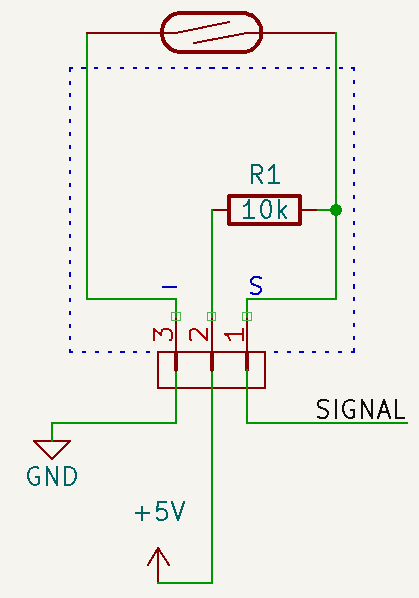
\includegraphics[width=.5\linewidth]{fig/Kontaktron-KY-021/polaczenie_modulu/podciagajacy.png}
  \label{fig:sub1}
  \caption{Wariant połączenia pull-up}
\end{subfigure}%
\begin{subfigure}{.5\textwidth}
  \centering
  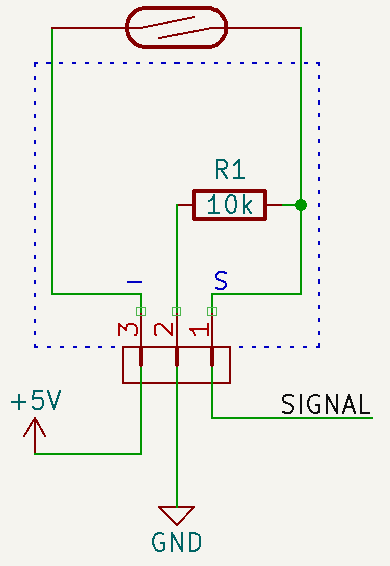
\includegraphics[width=.5\linewidth]{fig/Kontaktron-KY-021/polaczenie_modulu/sciagajacy.png}
  \label{fig:sub2}
  \caption{Wariant połączenia pull-down}
\end{subfigure}
\caption{Połączenie elektryczne}
\label{fig:test}
\end{figure}
\vspace{0.5cm}

\vspace{0.5cm}
\begin{table}[h!]
    \centering
    \begin{tabular}{|c|c|c|c|} 
        \hline
        \multicolumn{2}{|c|}{NUCELO-F746ZG} & \multicolumn{2}{c|}{SENSOR}  \\ 
        \hline
        Etykieta & Port i numer pinu       & Nr pinu & Etykieta           \\ 
        \hline
        D33      & PB0                     & 1       & S              \\
        +5V      & +5V                      & 2     &   \\
        GND      & GND                       & 3       & -              \\
        \hline
    \end{tabular}
    \caption{Konfiguracja - pull-up}
\end{table}
\vspace{0.5cm}

\vspace{0.5cm}
\begin{table}[h!]
    \centering
    \begin{tabular}{|c|c|c|c|} 
        \hline
        \multicolumn{2}{|c|}{NUCELO-F746ZG} & \multicolumn{2}{c|}{SENSOR}  \\ 
        \hline
        Etykieta & Port i numer pinu       & Nr pinu & Etykieta           \\ 
        \hline
        D33      & PB0                     & 1       & S              \\
        GND      & GND                      & 2     &   \\
        +5V     & +5V                      & 3       & -              \\
        \hline
    \end{tabular}
    \caption{Konfiguracja - pull-down}
\end{table}
\vspace{0.5cm}

% \subsection{Konfiguracja IOC}
% W CubeIDE zmieniono konfigurację pinu PB0 na GPIO\_Input.

% \vspace{0.5cm}
% \begin{figure}[H]
%     \centering
%     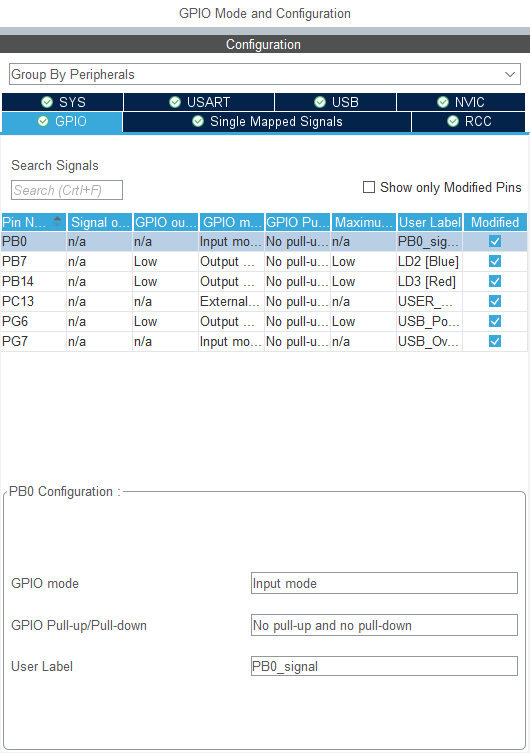
\includegraphics[width=9cm]{fig/Kontaktron-KY-021/polaczenie_modulu/IOC.PNG}
%     \caption{Konfiguracja GPIO mikrokotnrolera}
%     \label{fig:my_label}
% \end{figure}
% \vspace{0.5cm}

% \subsection{Oprogramowanie mikrokontrolera}
% Kod do podstawowej obsługi i monitorowania aktywności modułu KY-021 znajduje się w materiałach dodatkowych pod koniec rodziału.

\section{Prezentacja działania układu}
Złożony układ w konfiguracji pull-down i pull-up podłączono do mikrokontrolera NUCLEO-F746ZG z wgranym programem i ustawieniami z poprzednich podpunktów. W bibliografii znajduje się także nagranie pokazujące działanie modułu przy pomocy diody zielonej użytkownika LD1 \cite{youtube}.

% \vspace{0.5cm}
% \begin{figure}[H]
% \centering
% \begin{subfigure}{.5\textwidth}
%   \centering
%   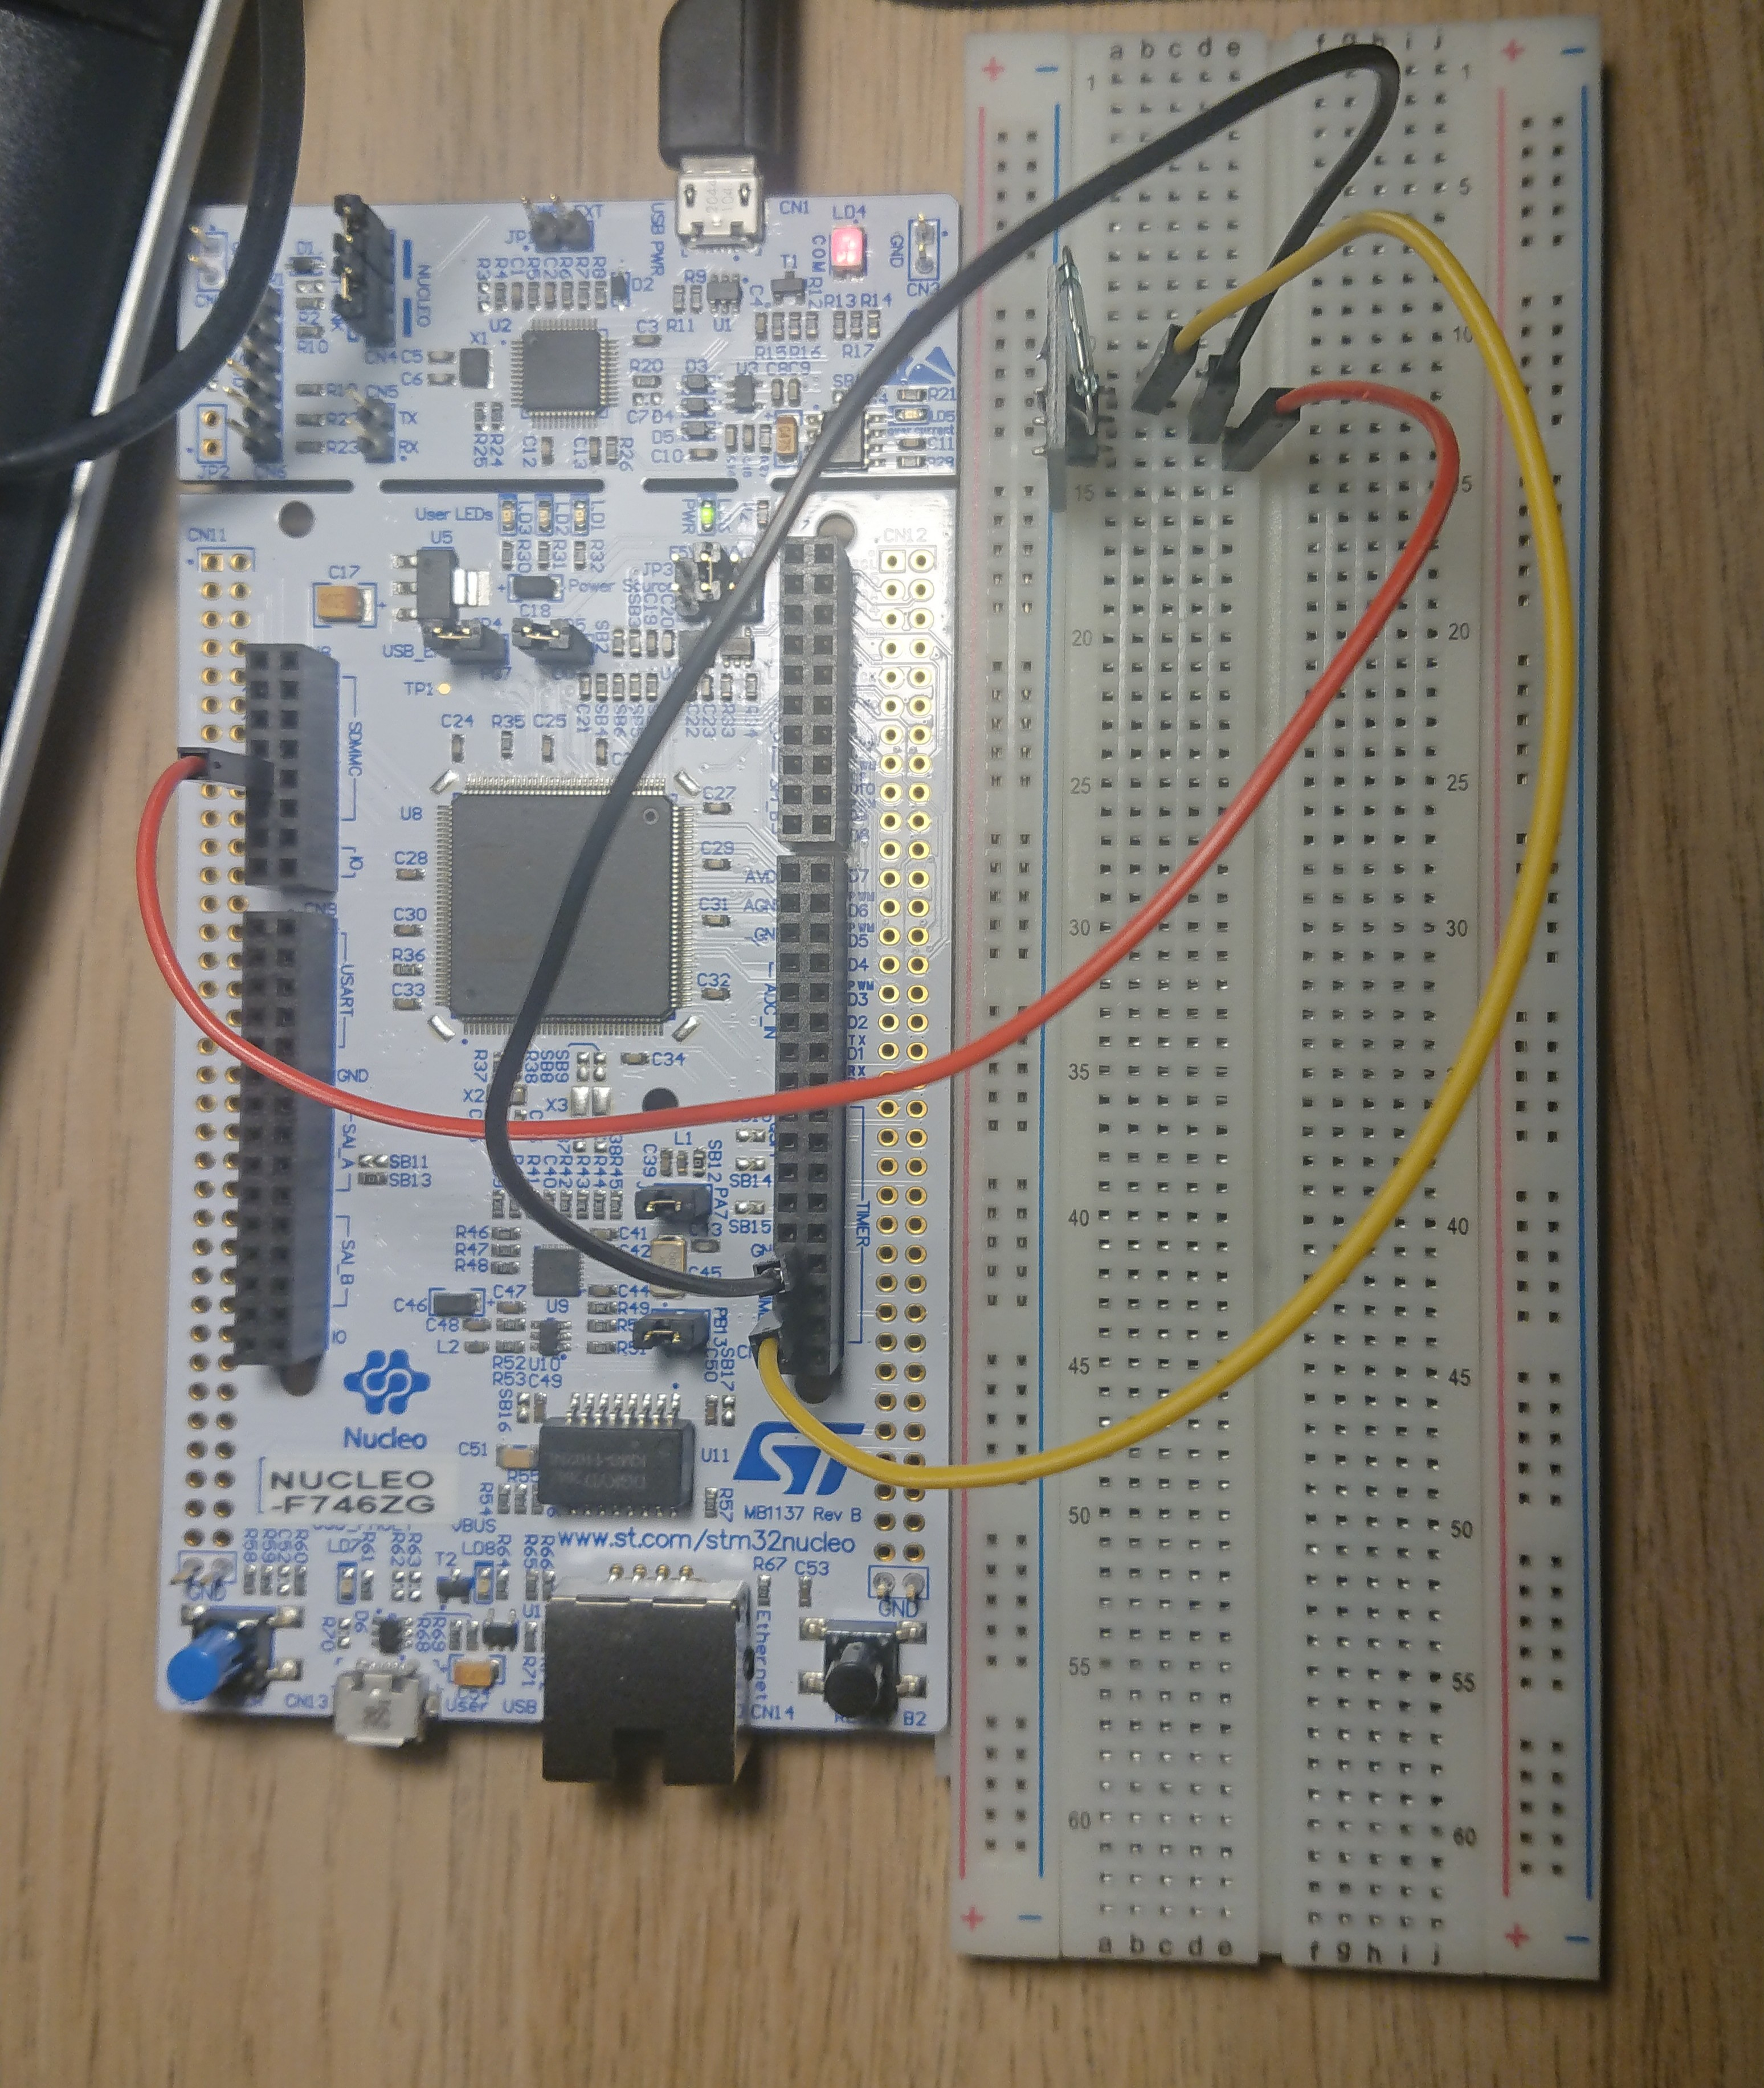
\includegraphics[width=.7\linewidth]{fig/Kontaktron-KY-021/działanie_ukladu/_20220331_005813.JPG}
%   \label{fig:sub1}
%   \caption{Wariant połączenia pull-down}
% \end{subfigure}%
% \begin{subfigure}{.5\textwidth}
%   \centering
%   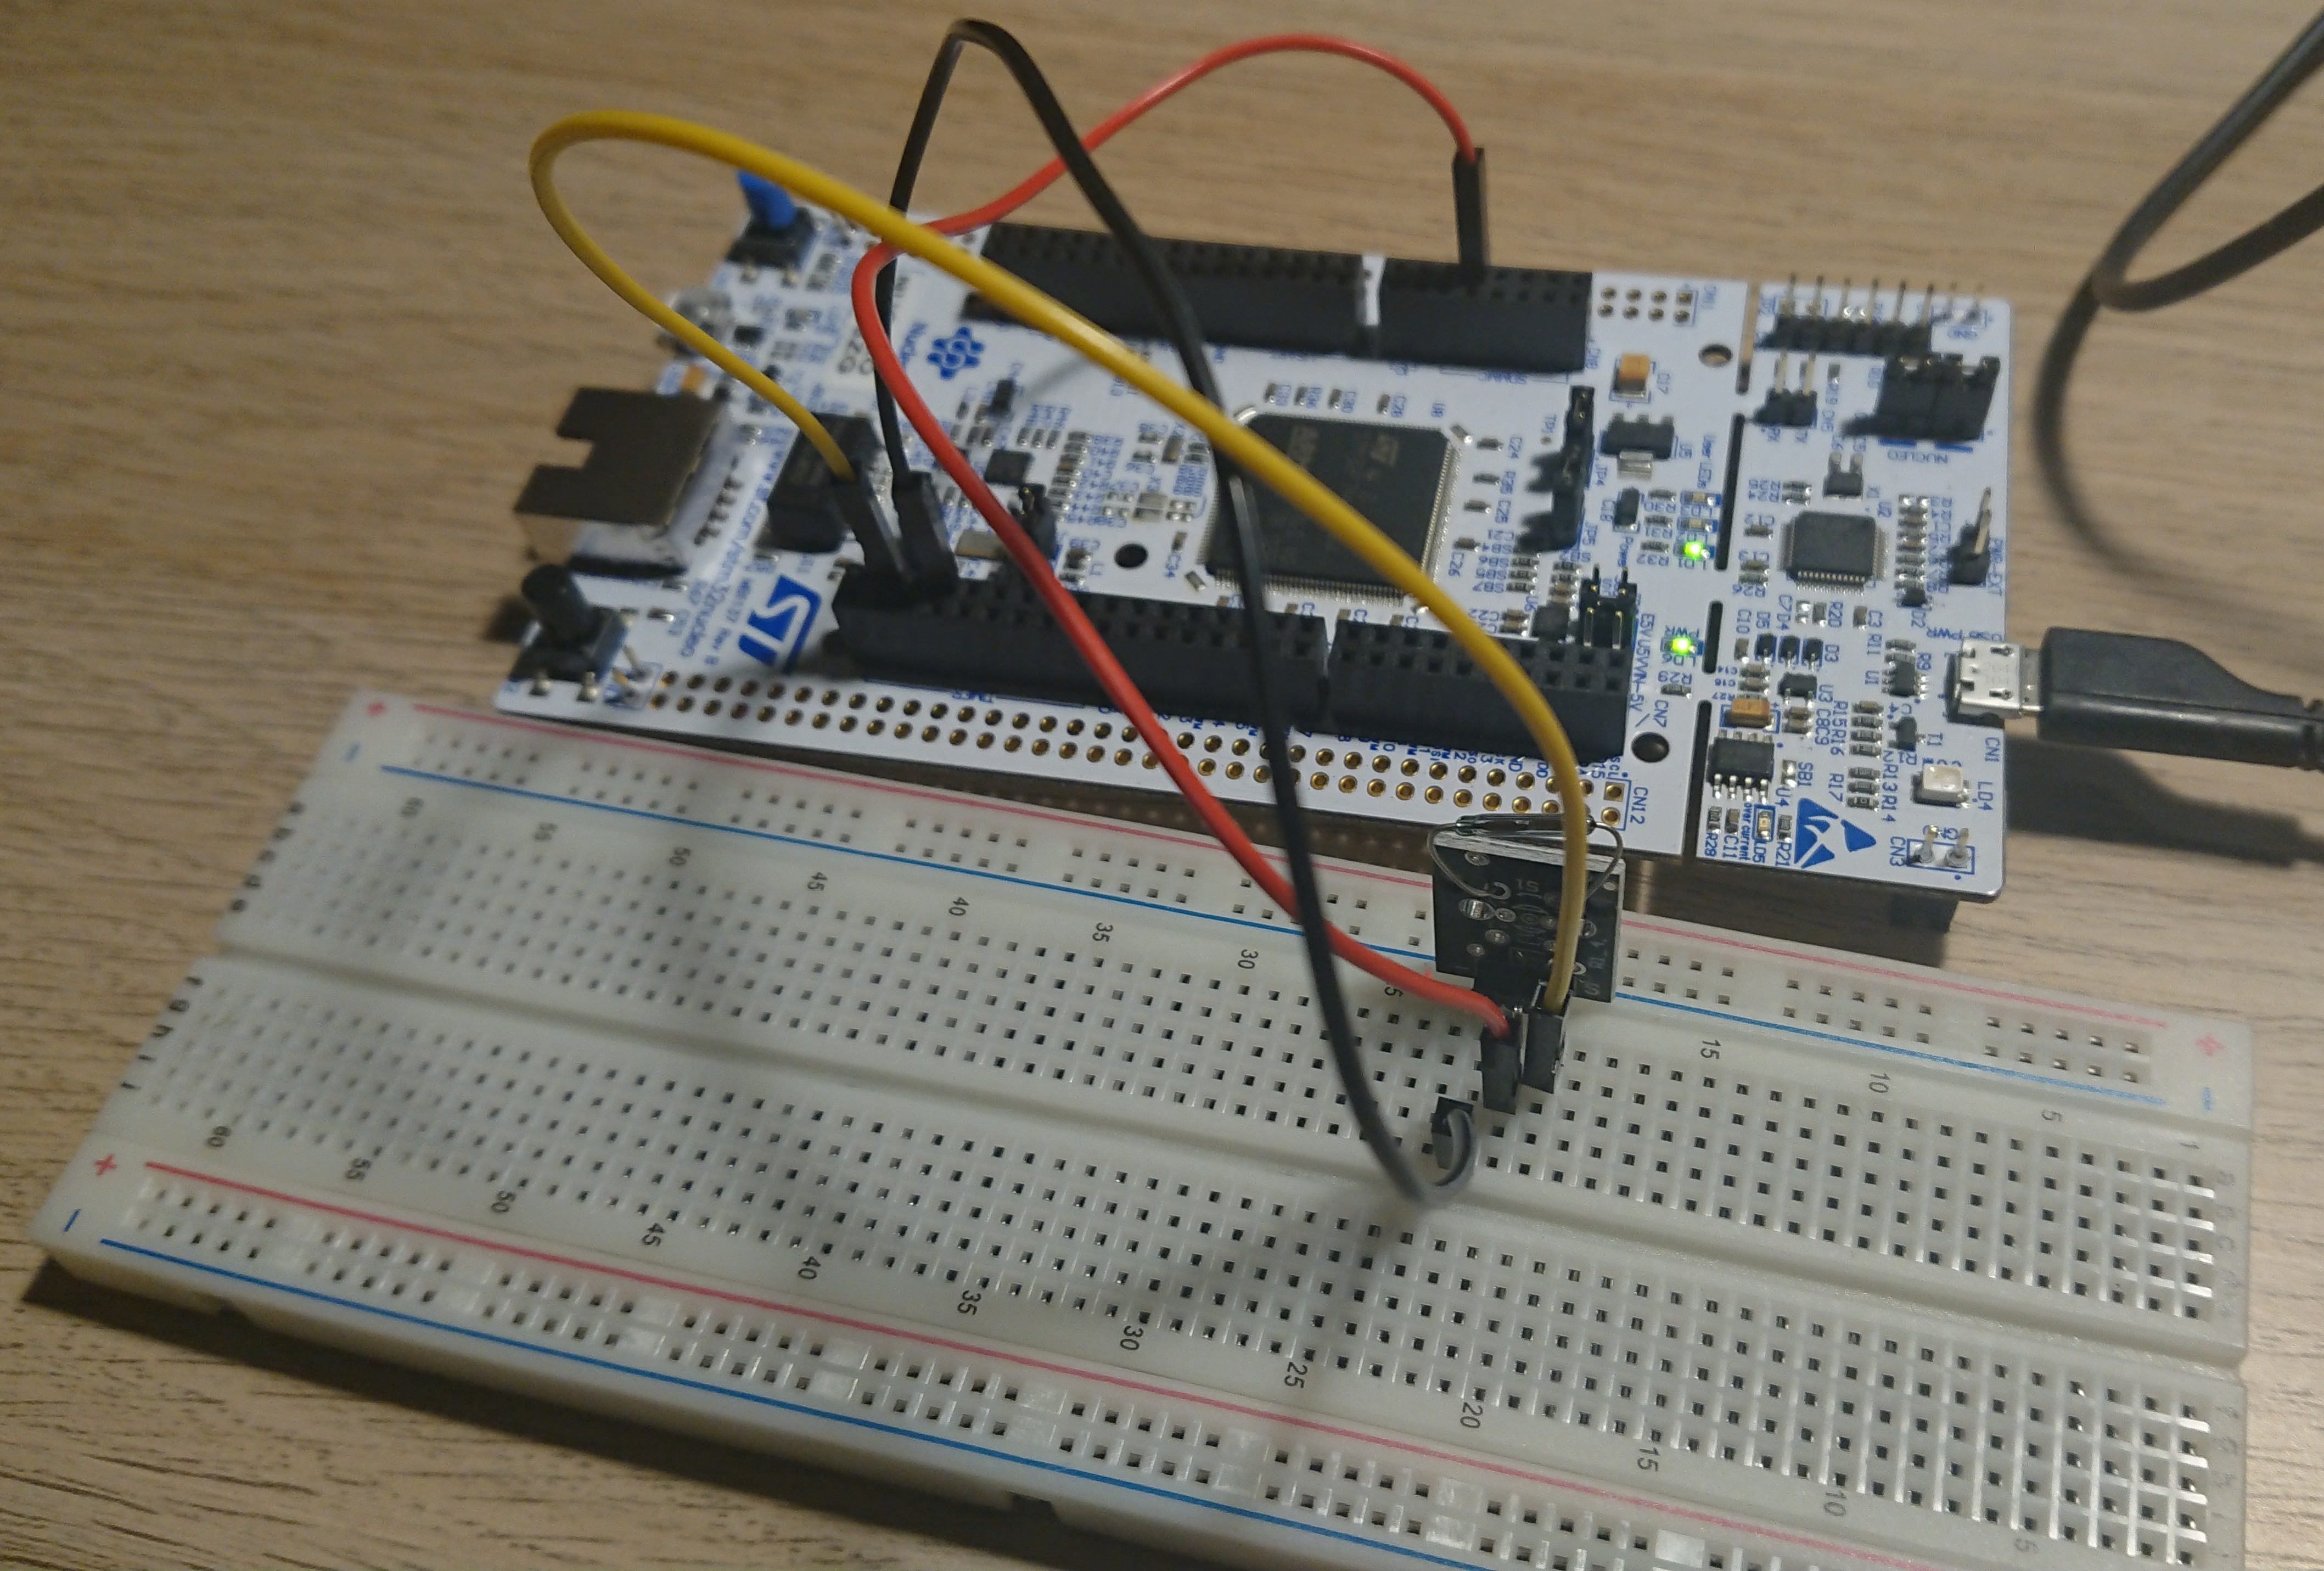
\includegraphics[width=.9\linewidth]{fig/Kontaktron-KY-021/działanie_ukladu/_20220331_010019.JPG}
%   \label{fig:sub2}
%   \caption{Wariant połączenia pull-up}
% \end{subfigure}
% \label{fig:test}
% \end{figure}
% \vspace{0.2cm}

\vspace{0.5cm}
\begin{figure}[H]
  \centering
  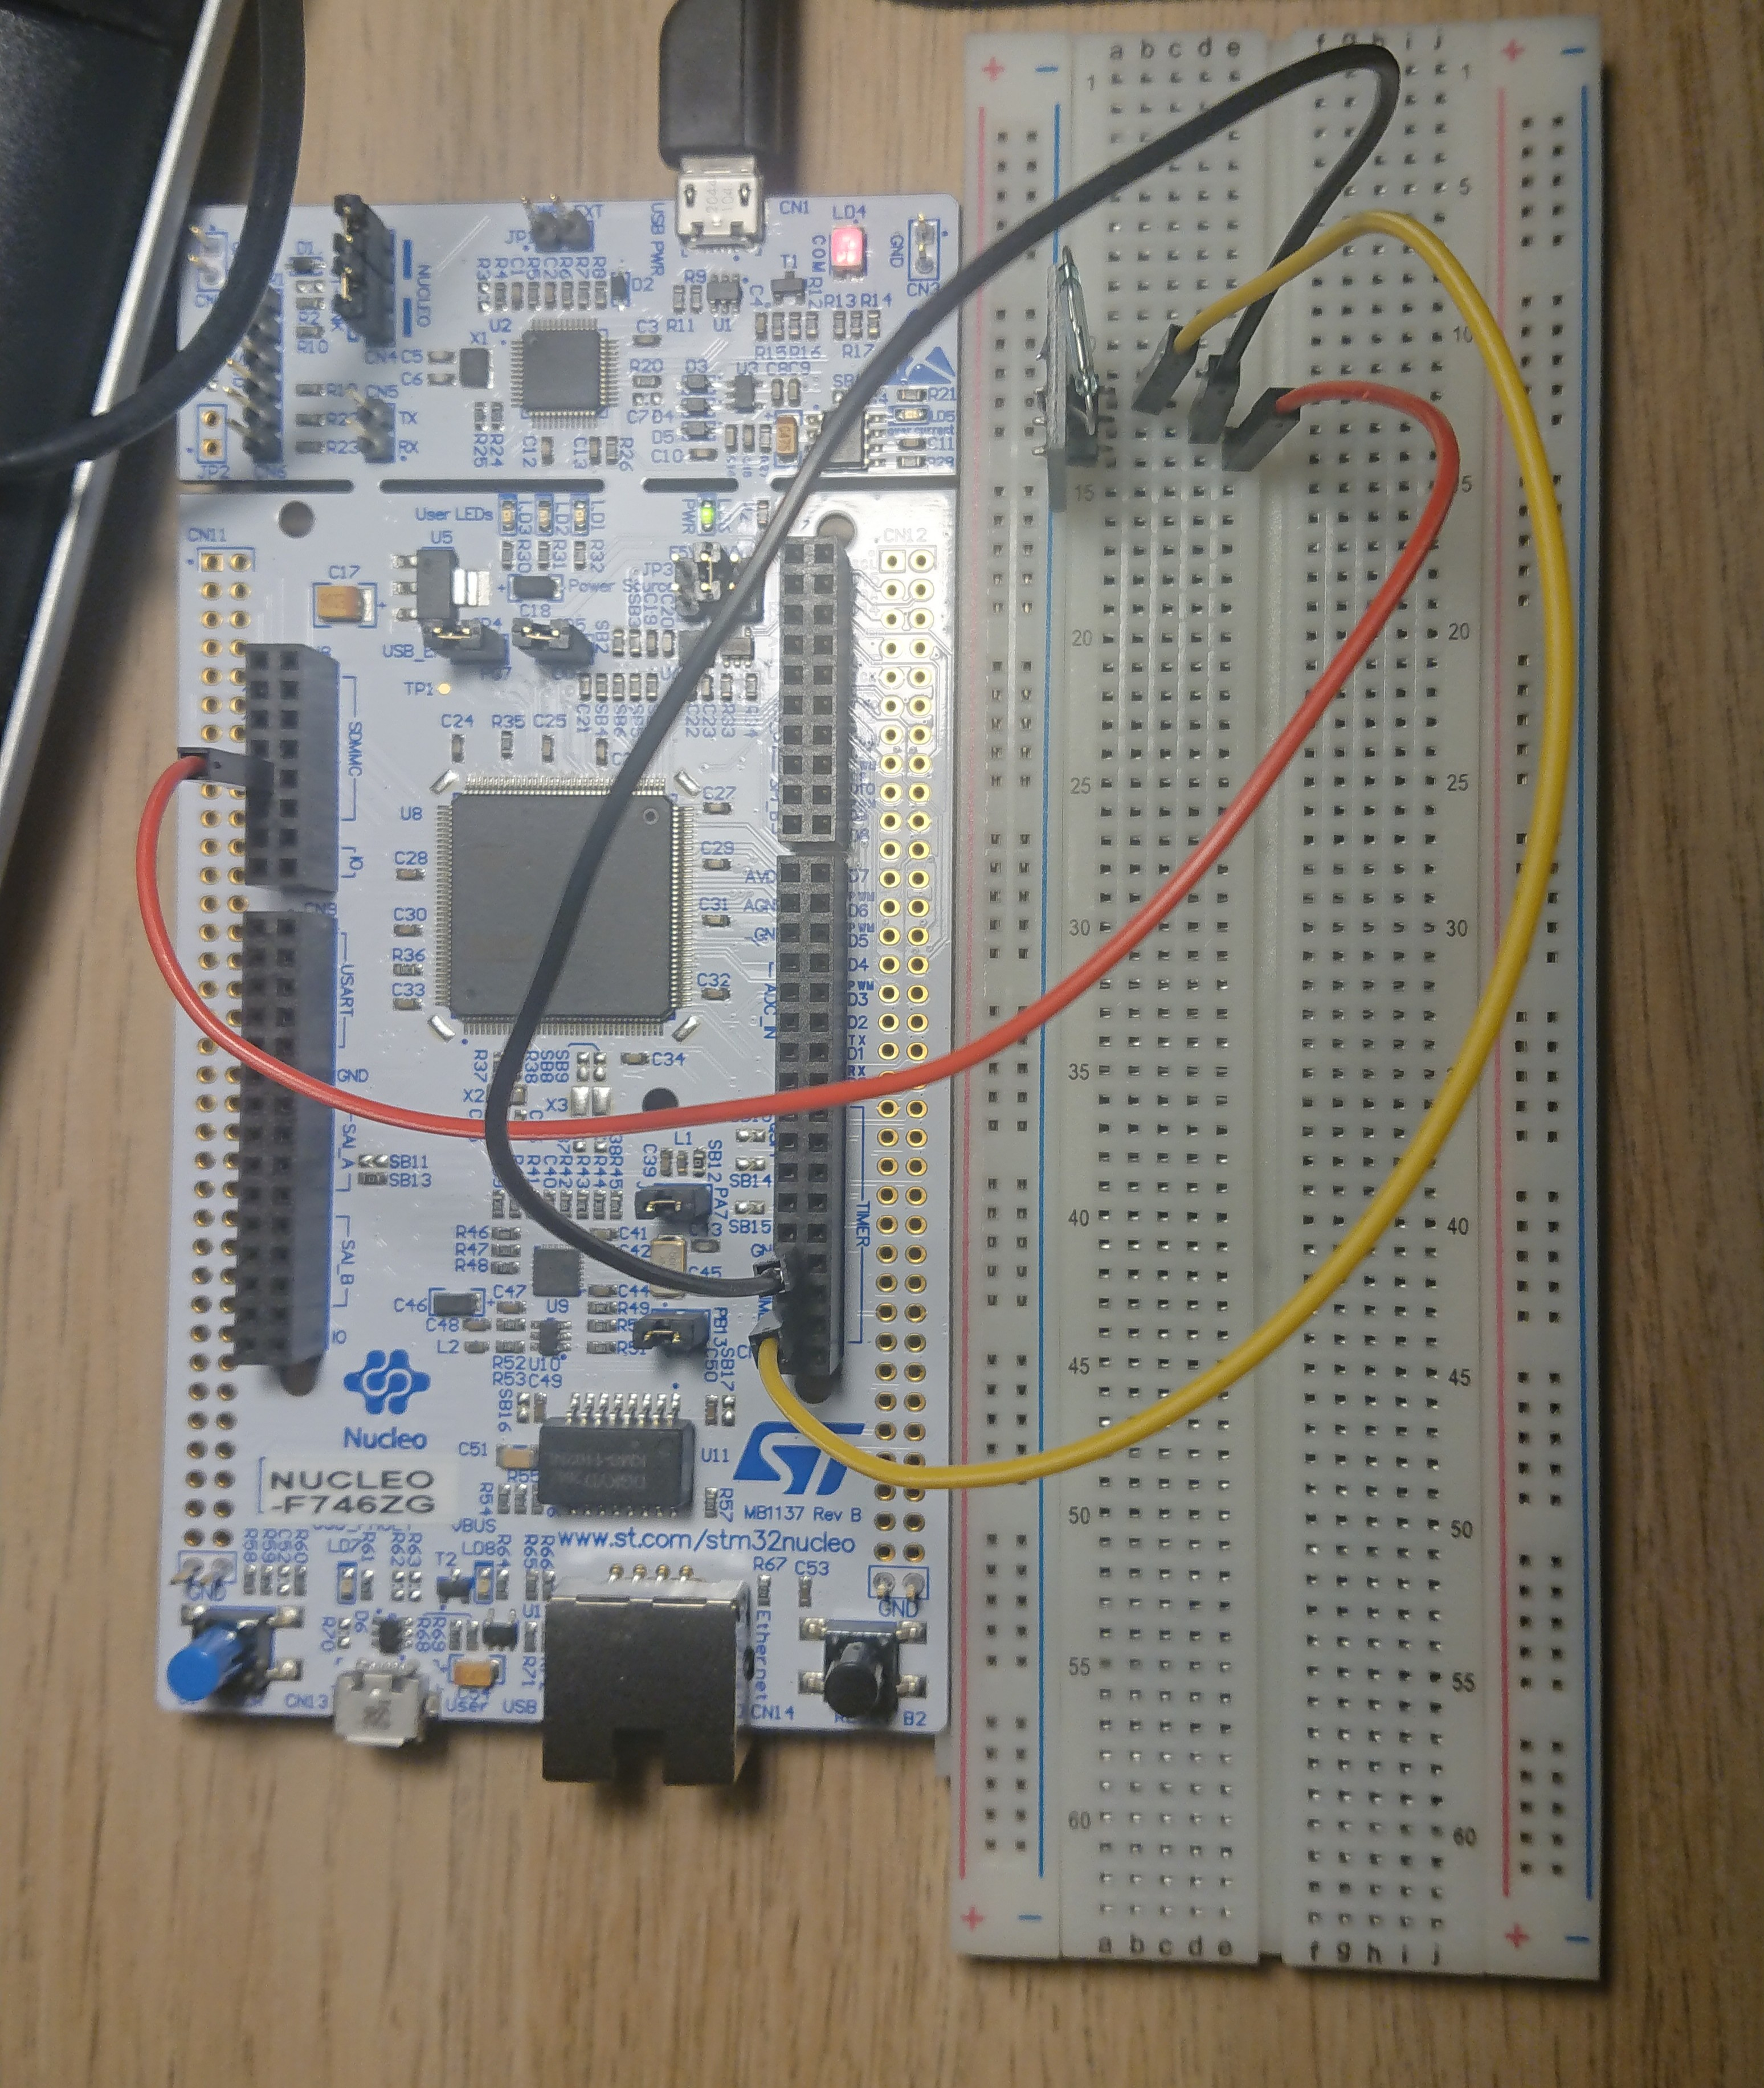
\includegraphics[width=.7\linewidth]{fig/Kontaktron-KY-021/działanie_ukladu/_20220331_005813.JPG}
  \label{fig:sub1}
  \caption{Wariant połączenia pull-down}
\end{figure}
\vspace{0.5cm}

\vspace{0.5cm}
\begin{figure}[H]
  \centering
  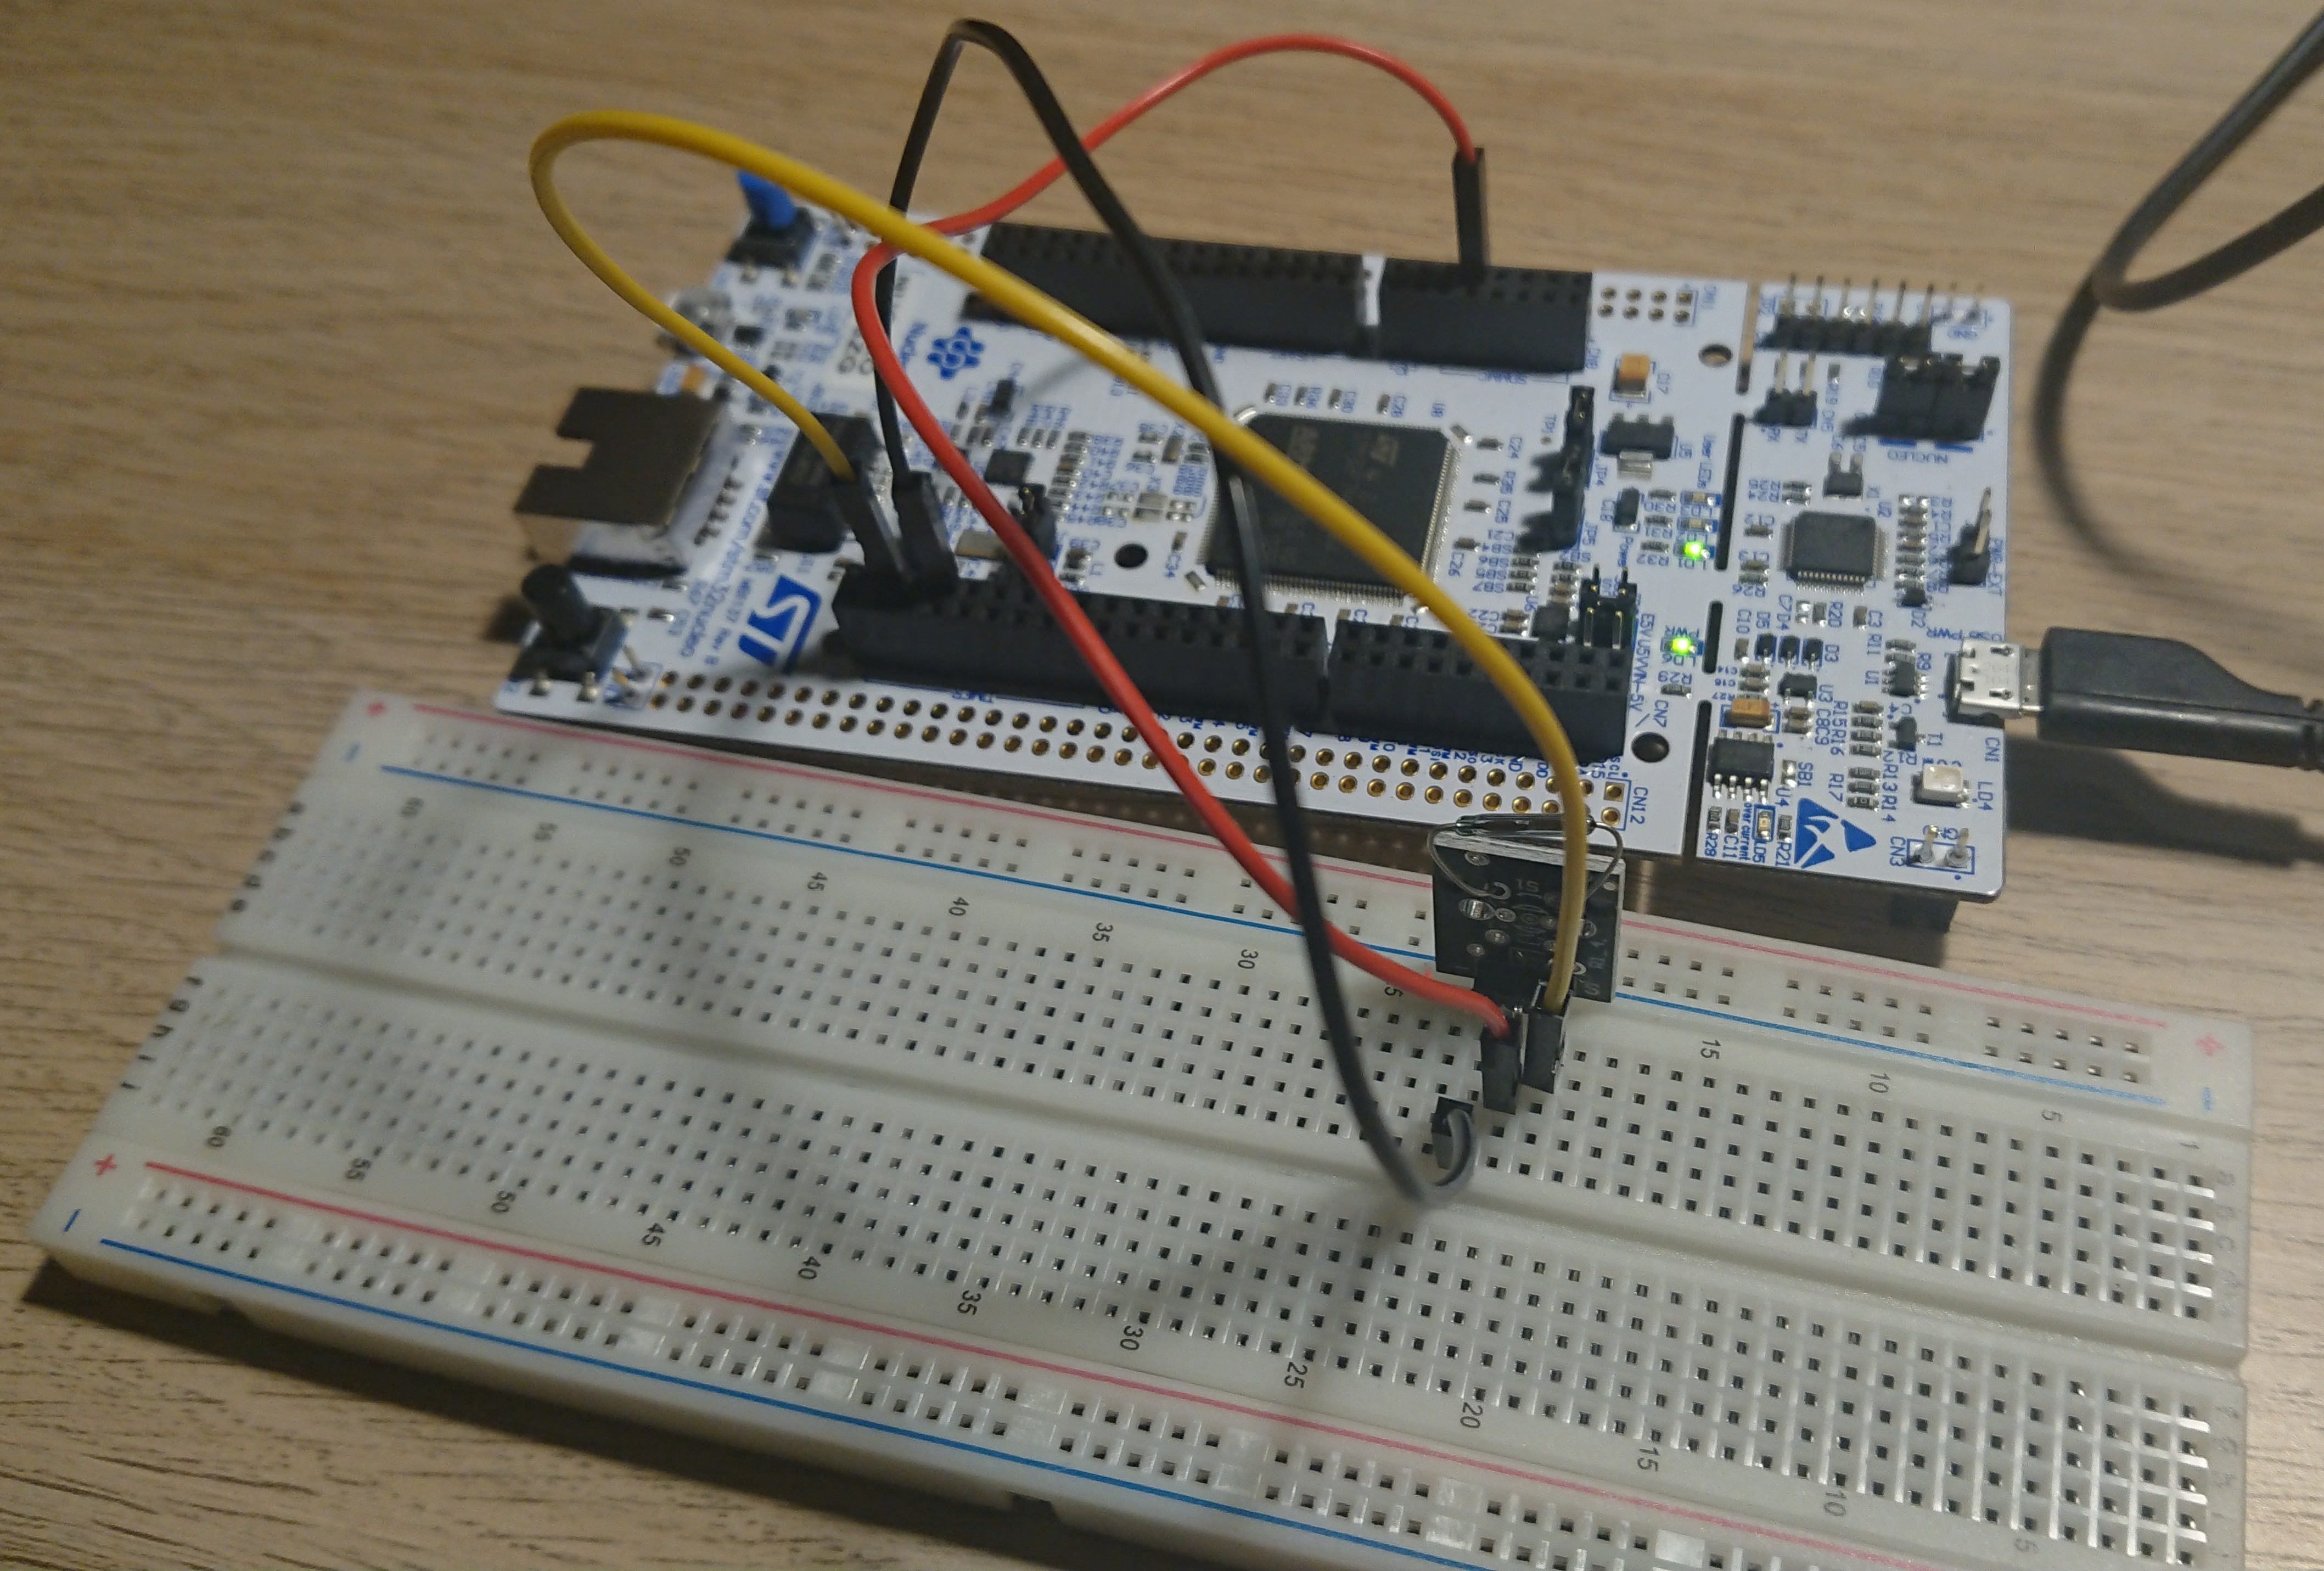
\includegraphics[width=.7\linewidth]{fig/Kontaktron-KY-021/działanie_ukladu/_20220331_010019.JPG}
  \label{fig:sub2}
  \caption{Wariant połączenia pull-up}
\end{figure}
\vspace{0.5cm}

% \vspace{0.2cm}
% \begin{figure}[H]
%     \centering
%     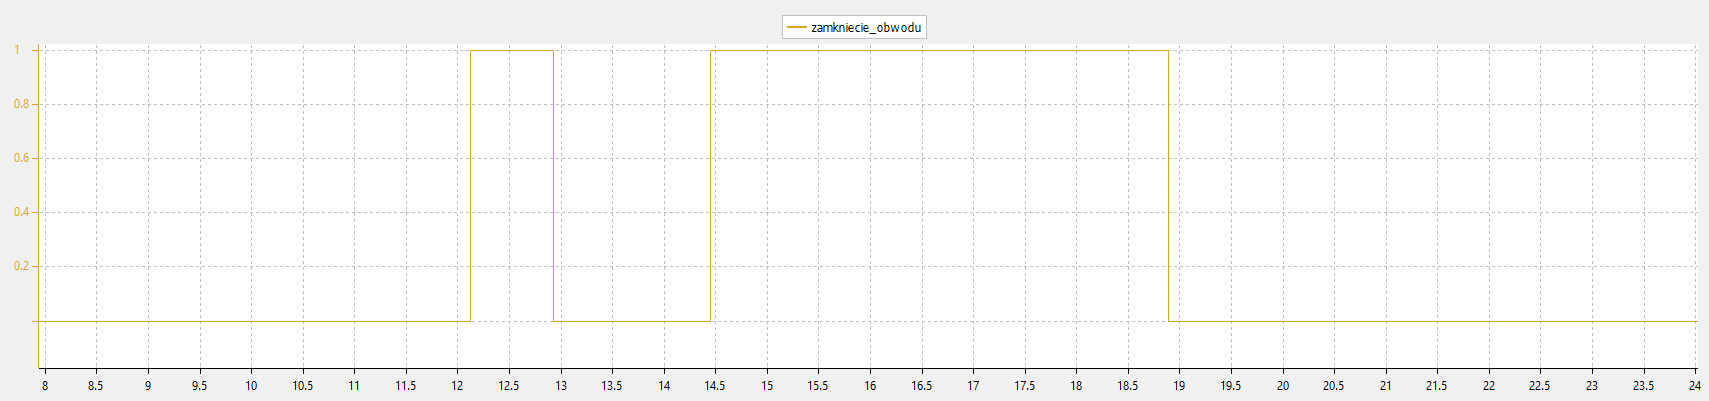
\includegraphics[width=1\textwidth]{fig/Kontaktron-KY-021/działanie_ukladu/swv.PNG}
%     \caption{Konfiguracja pull-down, zbliżenie magnesu powoduje zamknięcie obwodu i napływ prądu do pinu sygnałowego, jest to wykrywane jako stan wysoki (''1'').}
%     \label{fig:my_label}
% \end{figure}
% \vspace{0.2cm}

% \vspace{0.3cm}
% \begin{figure}[H]
%     \centering
%     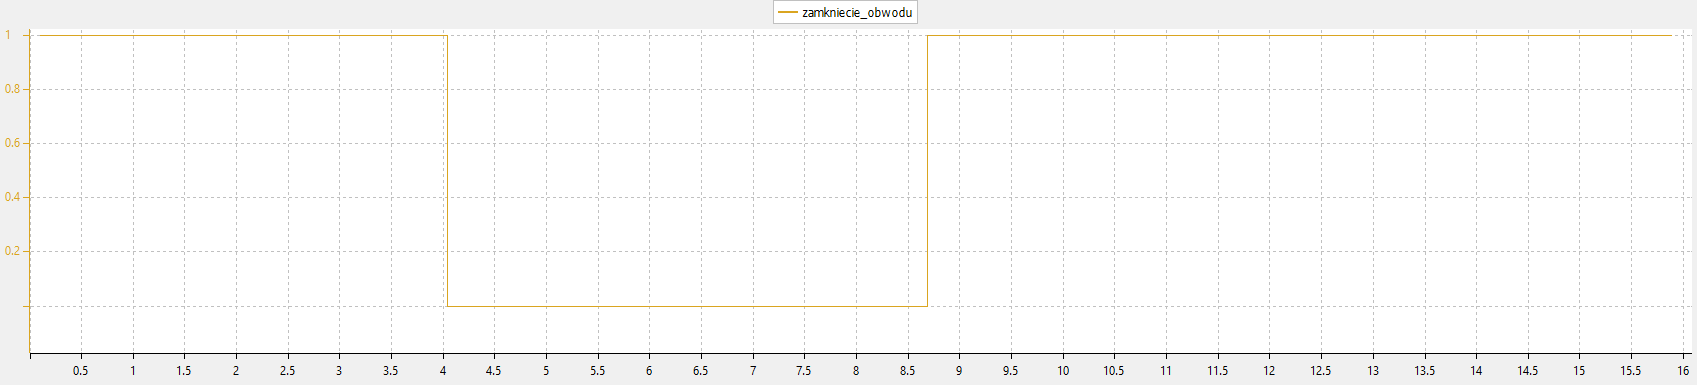
\includegraphics[width=1\textwidth]{fig/Kontaktron-KY-021/działanie_ukladu/swv2.PNG}
%     \caption{Konfiguracja pull-up, zbliżenie magnesu powoduje zamknięcie obwodu i zmniejszenie napływu prądu do pinu sygnałowego (część prądu popłynęła w stronę uziemienia), co jest wykrywane jako stan niski (''0'').}
%     \label{fig:my_label}
% \end{figure}
% \vspace{0.2cm}

%\newpage

\printbibliography[heading=bibintoc]

\end{document}